
\documentclass[twoside]{article}

\usepackage{lipsum} % Package to generate dummy text throughout this template


\usepackage[sc]{mathpazo} % Use the Palatino font
\usepackage[T1]{fontenc} % Use 8-bit encoding that has 256 glyphs
\linespread{1.05} % Line spacing - Palatino needs more space between lines
\usepackage{microtype} % Slightly tweak font spacing for aesthetics
\usepackage{graphicx}
\usepackage[hmarginratio=1:1,top=32mm,columnsep=20pt]{geometry} % Document margins
\usepackage{multicol} % Used for the two-column layout of the document
\usepackage[hang, small,labelfont=bf,up,textfont=it,up]{caption} % Custom captions under/above floats in tables or figures
\usepackage{booktabs} % Horizontal rules in tables
\usepackage{float} % Required for tables and figures in the multi-column environment - they need to be placed in specific locations with the [H] (e.g. \begin{table}[H])
\usepackage{hyperref} % For hyperlinks in the PDF

\usepackage{lettrine} % The lettrine is the first enlarged letter at the beginning of the text
\usepackage{paralist} % Used for the compactitem environment which makes bullet points with less space between them

\usepackage{abstract} % Allows abstract customization
\renewcommand{\abstractnamefont}{\normalfont\bfseries} % Set the "Abstract" text to bold
\renewcommand{\abstracttextfont}{\normalfont\small\itshape} % Set the abstract itself to small italic text

\usepackage{titlesec} % Allows customization of titles
\renewcommand\thesection{\Roman{section}} % Roman numerals for the sections
\renewcommand\thesubsection{\Roman{subsection}} % Roman numerals for subsections
\titleformat{\section}[block]{\large\scshape\centering}{\thesection.}{1em}{} % Change the look of the section titles
\titleformat{\subsection}[block]{\large}{\thesubsection.}{1em}{} % Change the look of the section titles

\usepackage{fancyhdr} % Headers and footers
\pagestyle{fancy} % All pages have headers and footers
\fancyhead{} % Blank out the default header
\fancyfoot{} % Blank out the default footer
\fancyhead[C]{Running title $\bullet$ November 2012 $\bullet$ Vol. XXI, No. 1} % Custom header text
\fancyfoot[RO,LE]{\thepage} % Custom footer text

%----------------------------------------------------------------------------------------
%	TITLE SECTION
%----------------------------------------------------------------------------------------

\title{\vspace{-15mm}\fontsize{24pt}{10pt}\selectfont\textbf{Pruning Gradient Boosted Oblivious Decision Trees}} % Article title

\author{
\large
\textsc{A. Rogozhnikov, A. Panin}
%\normalsize \href{mailto:justHeuristic@gmail.com}{john@smith.com} % Your email address
\vspace{-5mm}
}
\date{}

%----------------------------------------------------------------------------------------

\begin{document}

\maketitle % Insert title

\thispagestyle{fancy} % All pages have headers and footers

%----------------------------------------------------------------------------------------
%	ABSTRACT
%----------------------------------------------------------------------------------------

\begin{abstract}

\noindent This paper describes an approach to the problem of pruning the Gradient Boosted Oblivious Decision Trees that aims in maintaining the maximal quality of the full ensemble while removing most of the trees from it and adjusting the individual trees. The results are then evaluated by the ROC AUC score on the HIGGS dataset.

\end{abstract}

%----------------------------------------------------------------------------------------
%	ARTICLE CONTENTS
%----------------------------------------------------------------------------------------

\begin{multicols}{2} % Two-column layout throughout the main article text

\section{Introduction}

	One of the most popular method branches used in state of art machine learning applications is the inductive decision tree learning [1]. While the greedy decision tree composition methods are relatively computationaly inexpensive, they tend to show remarkable performance on datasets with numerous features of different origin. The decision trees are also used to perform feature selection [2] from the high dimensionality data for further use in more sophisticated models. One more obvious advantage of decision trees is their interpretability, as compared to most other approaches.
    

	Apart from the classical decision trees, there are several known alternative decision tree forms, and among them, the so called Oblivious Decision Trees (ODT) [3], that differ from classical ones in that they use the same splitting criterion in every node within a depth layer, thus in effect being decision tables.
    

	This simplification, while diminishing the individual efficiency of a trained ODT model, allows for a considerable speed up in the training algorithm runtime, thus increasing performance in ensemble models (typically bagging [4][5] or boosting[6][7] variations), that average the results from sets of decision trees to get the best quality.


%------------------------------------------------

\section{On Gradient Boosting}

The majority of approaches, suggested in the current paper, were inspired by and tested on the so called Gradient Boosted Decision Trees [7] ensemble model, that can be formally defined as a result of additive iterative gradient optimisation of the loss function.


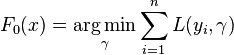
\includegraphics[width=120pt]{f1.png} 
\newline
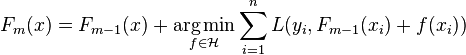
\includegraphics[width=200pt]{f2.png}


Fig.1 the formal gradient boosting definition

Here, F stands for the ensemble model, L is the loss function, H represents the model space (in this case, decision trees), f stands for a particular model within H, yi is the label of the ith training sample, n – total amount of samples, m – amount of gradient boosting optimization steps.

It should be of course noted, that the practical implementation of gradient boosting is swarming with countless heuristics from the domain of divine providence and/or the black magic. The above formulae are only presented to demonstrate the core principle of gradient boosting.

The advantages and drawbacks of the gradient boosted ODT are numerous, yet their analysis lies so far outside [8] the discourse universe of this article. What is more important to it, some practical applications demand that the decision making time of the final model stays low enough. Unless some other structurally faster approach is possible, the ensemble needs to be pruned efficiently to reach the required execution speed.

%------------------------------------------------

\section{Application example}

One such practical application might be the problem of binary signal/background classification of the event (particle collision) within the LHCb experiment [9]. LHC collides a bunch of protons every 50 nanoseconds, thus producing a gigantic influx of data ( approx.  ${2*10^7}$  events per second). The main objects of interest within the experiment are the very rare decays, while the rest of the data is generally uninteresting.

In order to filter out some of the obviously background events, LHC uses the multi-level trigger architecture, that filters out most of the data flow on each level. The low level triggers are removing the obvious background events, while the higher levels are increasing the precision even further by dealing with the events, approved by the lower level triggers, thus dealing with harder problem on smaller (yet still immense) data flow.

The possible application of Gradient Boosted ODT can be seen within the architecture of high level trigger within the LHCb detector.

%------------------------------------------------

%----------------------------------------------------------------------------------------
%	REFERENCE LIST
%----------------------------------------------------------------------------------------

\begin{thebibliography}{99} % Bibliography - this is intentionally simple in this template

\bibitem {b1}
Qiang Yang, Philip S. Yu, Zhou Zhihua, and David Hand et al "Top 10 algorithms in data mining", Knowledge and Information Systems 14.1: 1 - 37, 2008
\bibitem {b2}
H. Deng, G. Runger, "Feature Selection via Regularized Trees", Proceedings of the 2012 International Joint Conference on Neural Networks (IJCNN), IEEE, 2012
\bibitem {b3}
Kohavi, R. \& Li, C. (1995). Oblivious decision trees, graphs, and top-down pruning. In Proceedings of the Fourteenth International Joint Conference on Artificial Intelligence (pp. 1071 - 1077). San Mateo, CA: Morgan Kaufmann.
\bibitem {b4}
Breiman, L. (1996a). Bagging predictors. Machine Learning 26 (2), 123 - 140.
\bibitem {b5}
Breiman, L. Random forests. Machine Learning, 45(1):5 - 32, 2001
\bibitem {b6}
Freund, Y. \& Schapire, R. (1996). Experiments with a new boosting algorithm, Machine Learning: Proceedings of the Thirteenth International Conference, 148 - 156
\bibitem {b7}
Friedman, J. H. "Greedy Function Approximation: A Gradient Boosting Machine." (February 1999)
\bibitem {b8}
A. Augusto Alves Jr. et al. (LHCb Collaboration) (2008). "The LHCb Detector at the LHC". Journal of Instrumentation 3 (8): S08005. (Full design documentation).

 
\end{thebibliography}

%----------------------------------------------------------------------------------------

\end{multicols}

\end{document}